% !TeX spellcheck = en_GB
%%%%%%%%%%%%%%%%%%%%%%%%%%%%%%%%%%%%%%%%%%%%%%%%%%%%%%%%%%%%%%%%%%%%%%%%%%%%%%%%
%\documentclass[handout]{beamer}\mode<handout>{\usetheme{default}}
%
\documentclass[presentation]{beamer}\mode<presentation>{\usetheme{AMSBolognaFC}}
%\documentclass[handout]{beamer}\mode<handout>{\usetheme{AMSBolognaFC}}
% \setbeamertemplate{bibliography item}{\insertbiblabel}
%%%%%%%%%%%%%%%%%%%%%%%%%%%%%%%%%%%%%%%%%%%%%%%%%%%%%%%%%%%%%%%%%%%%%%%%%%%%%%%%
\usepackage[english]{babel}
\usepackage[utf8]{inputenc}
% version
\newcommand{\versionmajor}{1}
\newcommand{\versionminor}{0}
\newcommand{\versionpatch}{0}
\newcommand{\version}{\versionmajor.\versionminor.\versionpatch}
%
\usepackage{cilc-2022-logic-api-ml-talk}
%%%%%%%%%%%%%%%%%%%%%%%%%%%%%%%%%%%%%%%%%%%%%%%%%%%%%%%%%%%%%%%%%%%%%%%%%%%%%%%%
\title[Logic API for ML]{
    % same title of the presented paper
    Logic Programming library for Machine Learning
}
%
\subtitle{API design and prototype}
%
% same authors order of the presented paper
\author[\sspeaker{Ciatto}, Castigliò, Calegari]{
	\speaker{Giovanni Ciatto}$^{*}$ % empth the presenting author
	\and
	Matteo Castigliò$^{\dagger}$
	\and
	Roberta Calegari$^{\S}$
	\\
    \texttt{\{$^{*}$giovanni.ciatto, $^{\S}$roberta.calegari\}@unibo.it}
    \\
    $^{\dagger}$\texttt{matteo.castiglio@studio.unibo.it}
}
%
\institute[UniBo]{
    $^{*}$Dipartimento di Informatica -- Scienza e Ingegneria (DISI)
    \\
    $^{\S}$Alma Mater Research Institute for Human Centered AI (AlmaAI)
    \\
    \textsc{Alma Mater Studiorum} -- Università di Bologna
}
%
\date[CILC, 2022]{
	$37^{th}$ Italian Conference on Computational Logic (CILC)
	\\
	July 1, 2022, Bologna (Italy)
}

%%%%%%%%%%%%%%%%%%%%%%%%%%%%%%%%%%%%%%%%%%%%%%%%%%%%%%%%%%%%%%%%%%%%%%%%%%%%%%%%
\begin{document}
%%%%%%%%%%%%%%%%%%%%%%%%%%%%%%%%%%%%%%%%%%%%%%%%%%%%%%%%%%%%%%%%%%%%%%%%%%%%%%%%

%\\\\\\\\\\\\\\\\\\\\\
\frame{\titlepage}
%\\\\\\\\\\\\\\\\\\\\\

%===============================================================================
\section{Context, Motivation, \& Goals}
%===============================================================================

%\\\\\\\\\\\\\\\\\\\\\
\begin{frame}[c]{Context}

    \begin{itemize}
        \item Prolog is the most prominent LP technology\ccite{prolog50years-tplp}
        %
        \begin{itemize}
            \item used to implement other logic-based technologies\ccite{lptech4mas-jaamas35}
        \end{itemize}

        \vfill

        \item Plenty of libraries supporting ML in mainstream languages
        %
        \begin{itemize}
            \item main features: training, (de)serialising, or using ML predictors
            %
            \begin{itemize}
                \item[eg] Scikit-Learn or Tensorflow for Python
                \item[eg] Smile or \deeplearningforj{} on the JVM
            \end{itemize}
        \end{itemize}

        \vfill

        \item Poor interoperability among LP and ML
        %
        \begin{itemize}
            \item mostly due to the lack of technologies bridging them
            \item arguably slowing down research about hybrid systems
        \end{itemize}
    \end{itemize}
\end{frame}
%\\\\\\\\\\\\\\\\\\\\\

%\\\\\\\\\\\\\\\\\\\\\
\begin{frame}[c]{Motivation}
    \begin{itemize}
        \item Need to fill the (technological) gap among ML and LP
        %
        \begin{itemize}
            \item especially for what concerns the ``LP calls ML'' case
        \end{itemize}

        \vfill

        \item Support the exploitation of ML predictors in LP
        %
        \begin{itemize}
            \item[eg] for training, (de)serialising, or using them
        \end{itemize}

        \vfill

        \item Enable the exploitation of trained predictors as logic predicates

        \vfill

        \item Support the implementation of hybrid systems
         %
         \begin{itemize}
            \item[ie] where symbolic AI is used to govern or combine sub-symbolic predictors
        \end{itemize}

    \end{itemize}
\end{frame}
%\\\\\\\\\\\\\\\\\\\\\

%\\\\\\\\\\\\\\\\\\\\\
\begin{frame}{Goal of the Paper}

    \begin{enumerate}
        \item Propose a logic API for ML
        %
        \begin{itemize}
            \item[ie] a set of logic predicates for working ML, in LP
            \item covering all phases of a ML workflow
        \end{itemize}

        \vfill

        \item Design a technological architecture for re-using existing ML libraries

        \vfill

        \item Select technologies for prototyping the API

        \vfill

        \item Highlight the (expected) benefits
    \end{enumerate}

\end{frame}
%\\\\\\\\\\\\\\\\\\\\\

%===============================================================================
\section{Background}
%===============================================================================

%\\\\\\\\\\\\\\\\\\\\\
\begin{frame}%[allowframebreaks]
\frametitle{General Supervised Learning Workflow}

    \begin{center}
        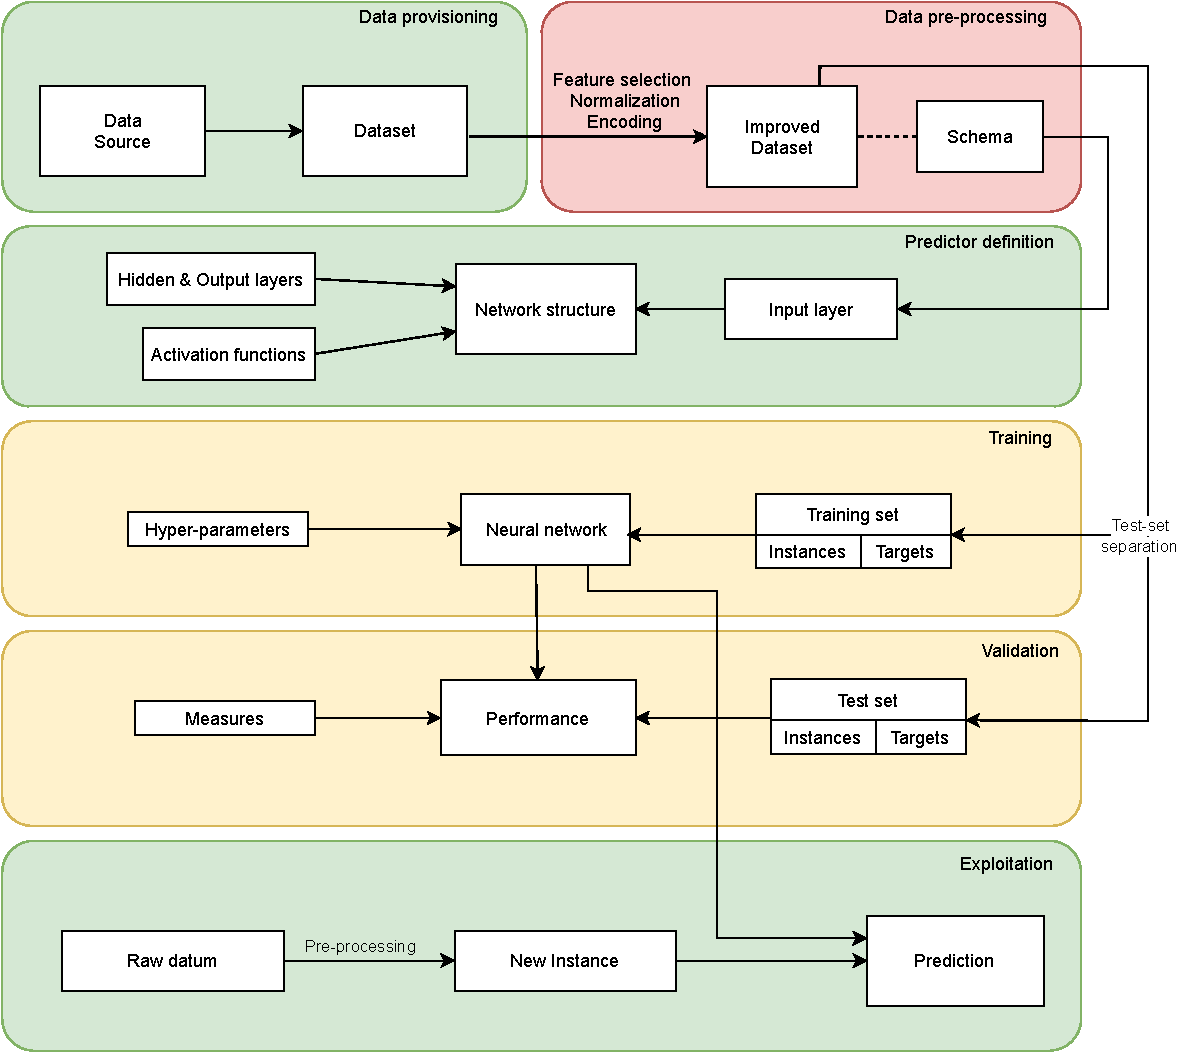
\includegraphics[width=.7\linewidth]{figures/phases1.pdf}
    \end{center}

\end{frame}
%\\\\\\\\\\\\\\\\\\\\\

\subsection{The \twopkt{} Logic Ecosystem}

\begin{frame}{Overview}
    \begin{block}{The \twopkt{} project \hfill (\url{https://github.com/tuProlog/2p-kt})}
        \begin{itemize}
            \item Kotlin-based implementation of a logic ecosystem
            \item multi-platform, multi-OS, multi-paradigm
        \end{itemize}
    \end{block}

    \begin{center}
        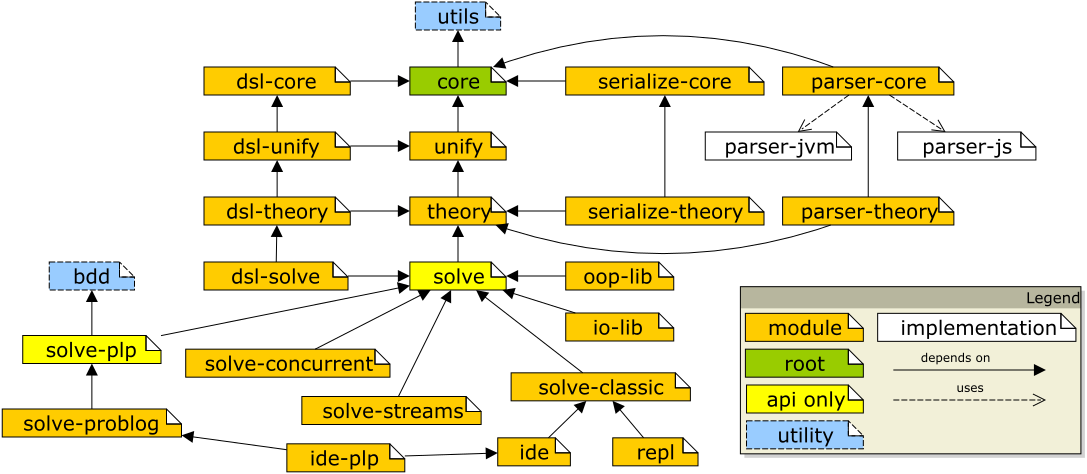
\includegraphics[width=.7\linewidth]{figures/project-map.png}
    \end{center}

    \vspace{-.5cm}

    \begin{multicols}{2}
        \begin{itemize}\small
            \item knowledge representation

            \item \ldots and storage

            \item \ldots and parsing/presentation

            \item Prolog-like inference support
            %
            \item \ldots or concurrent / probabilistic

            \item LP--OOP interoperability
        \end{itemize}
    \end{multicols}
\end{frame}

\begin{frame}{\twopkt{}'s General API for Logic Resolution\ccite{2pkt-jelia2021}}

    \begin{columns}
        \begin{column}{.49\linewidth}
            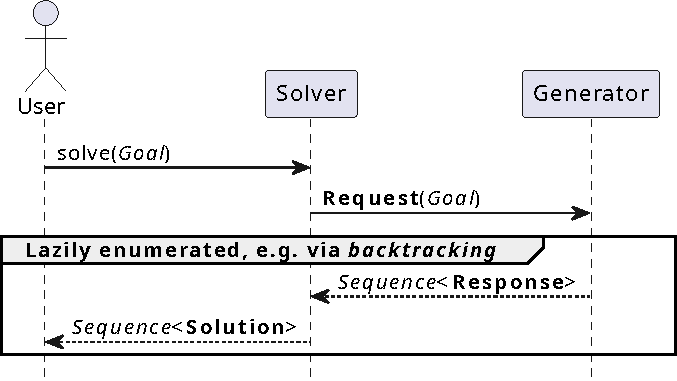
\includegraphics[width=\linewidth]{figures/primitive-usage.pdf}
        \end{column}
        \begin{column}{.49\linewidth}
            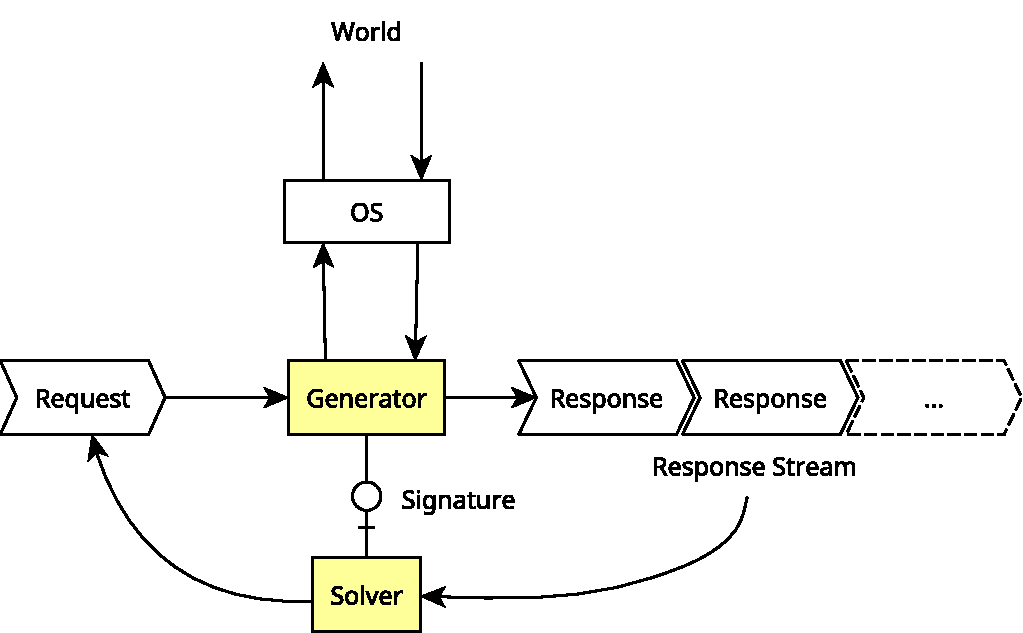
\includegraphics[width=\linewidth]{figures/generator.pdf}
        \end{column}
    \end{columns}

    \vfill

    \begin{itemize}
        \item Logic solvers as \alert{oracles} queried by users

        \vfill

        \item Generators as \alert{gateways} towards the external world
    \end{itemize}
\end{frame}

\section{Contributions}

\subsection{Expected benefits}

%\\\\\\\\\\\\\\\\\\\\\
\begin{frame}%[allowframebreaks]
\frametitle{Overview on expected benefits}

    \begin{itemize}
        \item Hybrid reasoning

        \item Declarative ML

        \item Symbolic data sources

        \item Model selection via resolution

    \end{itemize}

\end{frame}
%\\\\\\\\\\\\\\\\\\\\\

%\\\\\\\\\\\\\\\\\\\\\
\begin{frame}%[allowframebreaks]
    \frametitle{Hybrid reasoning}

    \begin{itemize}
        \item treating trained ML predictors as ordinary logic predicates
        \item hence enabling the combined exploitation of LP and ML
    \end{itemize}

    \prologimport{listings/hybrid-predictor.pl}

\end{frame}
%\\\\\\\\\\\\\\\\\\\\\

%\\\\\\\\\\\\\\\\\\\\\
\begin{frame}%[allowframebreaks]
    \frametitle{Declarative ML}

    \begin{itemize}
        \item use logic programs as declarative specification for ML aspects
    \end{itemize}

    \prologimport{listings/neural-network-declare.pl}

\end{frame}
%\\\\\\\\\\\\\\\\\\\\\

%\\\\\\\\\\\\\\\\\\\\\
\begin{frame}%[allowframebreaks]
    \frametitle{Symbolic data sources}

    \begin{itemize}
        \item use logic theories as datasets, and train predictors upon them
    \end{itemize}

    \prologimport[basicstyle=\tiny\ttfamily]{listings/logic-dataset-loading.pl}

\end{frame}
%\\\\\\\\\\\\\\\\\\\\\

%\\\\\\\\\\\\\\\\\\\\\
\begin{frame}[allowframebreaks]
    \frametitle{Model selection via resolution}

    \begin{itemize}
        \item exploit the non-determinism of resolution explore all possible choices
    \end{itemize}

    \prologimport%[basicstyle=\tiny\ttfamily]
    {listings/training.pl}

\end{frame}
%\\\\\\\\\\\\\\\\\\\\\

\subsection{Architectural Overview}

%\\\\\\\\\\\\\\\\\\\\\
\begin{frame}%[allowframebreaks]
    \frametitle{Most relevant components}

    \begin{columns}
        \column{.44\linewidth}
        \centering
        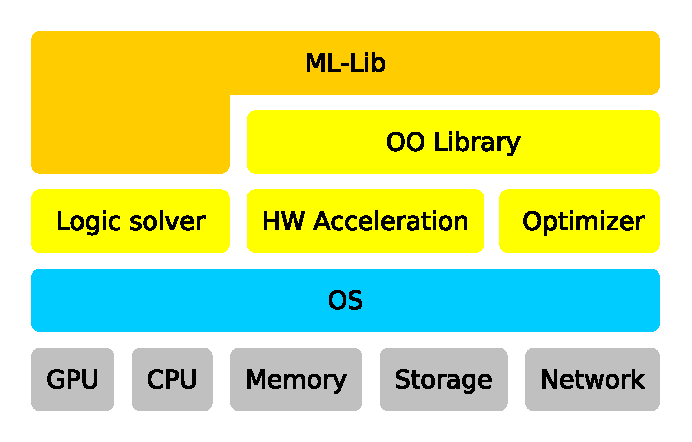
\includegraphics[width=\linewidth]{figures/layers.pdf}
        \column{.56\linewidth}
        \begin{itemize}
            \item a library of logic predicates (\mllib)
            \item some underlying OOP library for ML
            \item some underlying LP facility
            %
            \begin{itemize}
                \item supporting OOP-interoperability
            \end{itemize}
        \end{itemize}
    \end{columns}

\end{frame}
%\\\\\\\\\\\\\\\\\\\\\

\subsection{Main logic API}

%\\\\\\\\\\\\\\\\\\\\\
\begin{frame}%[allowframebreaks]
    \frametitle{About the \mllib{}}

    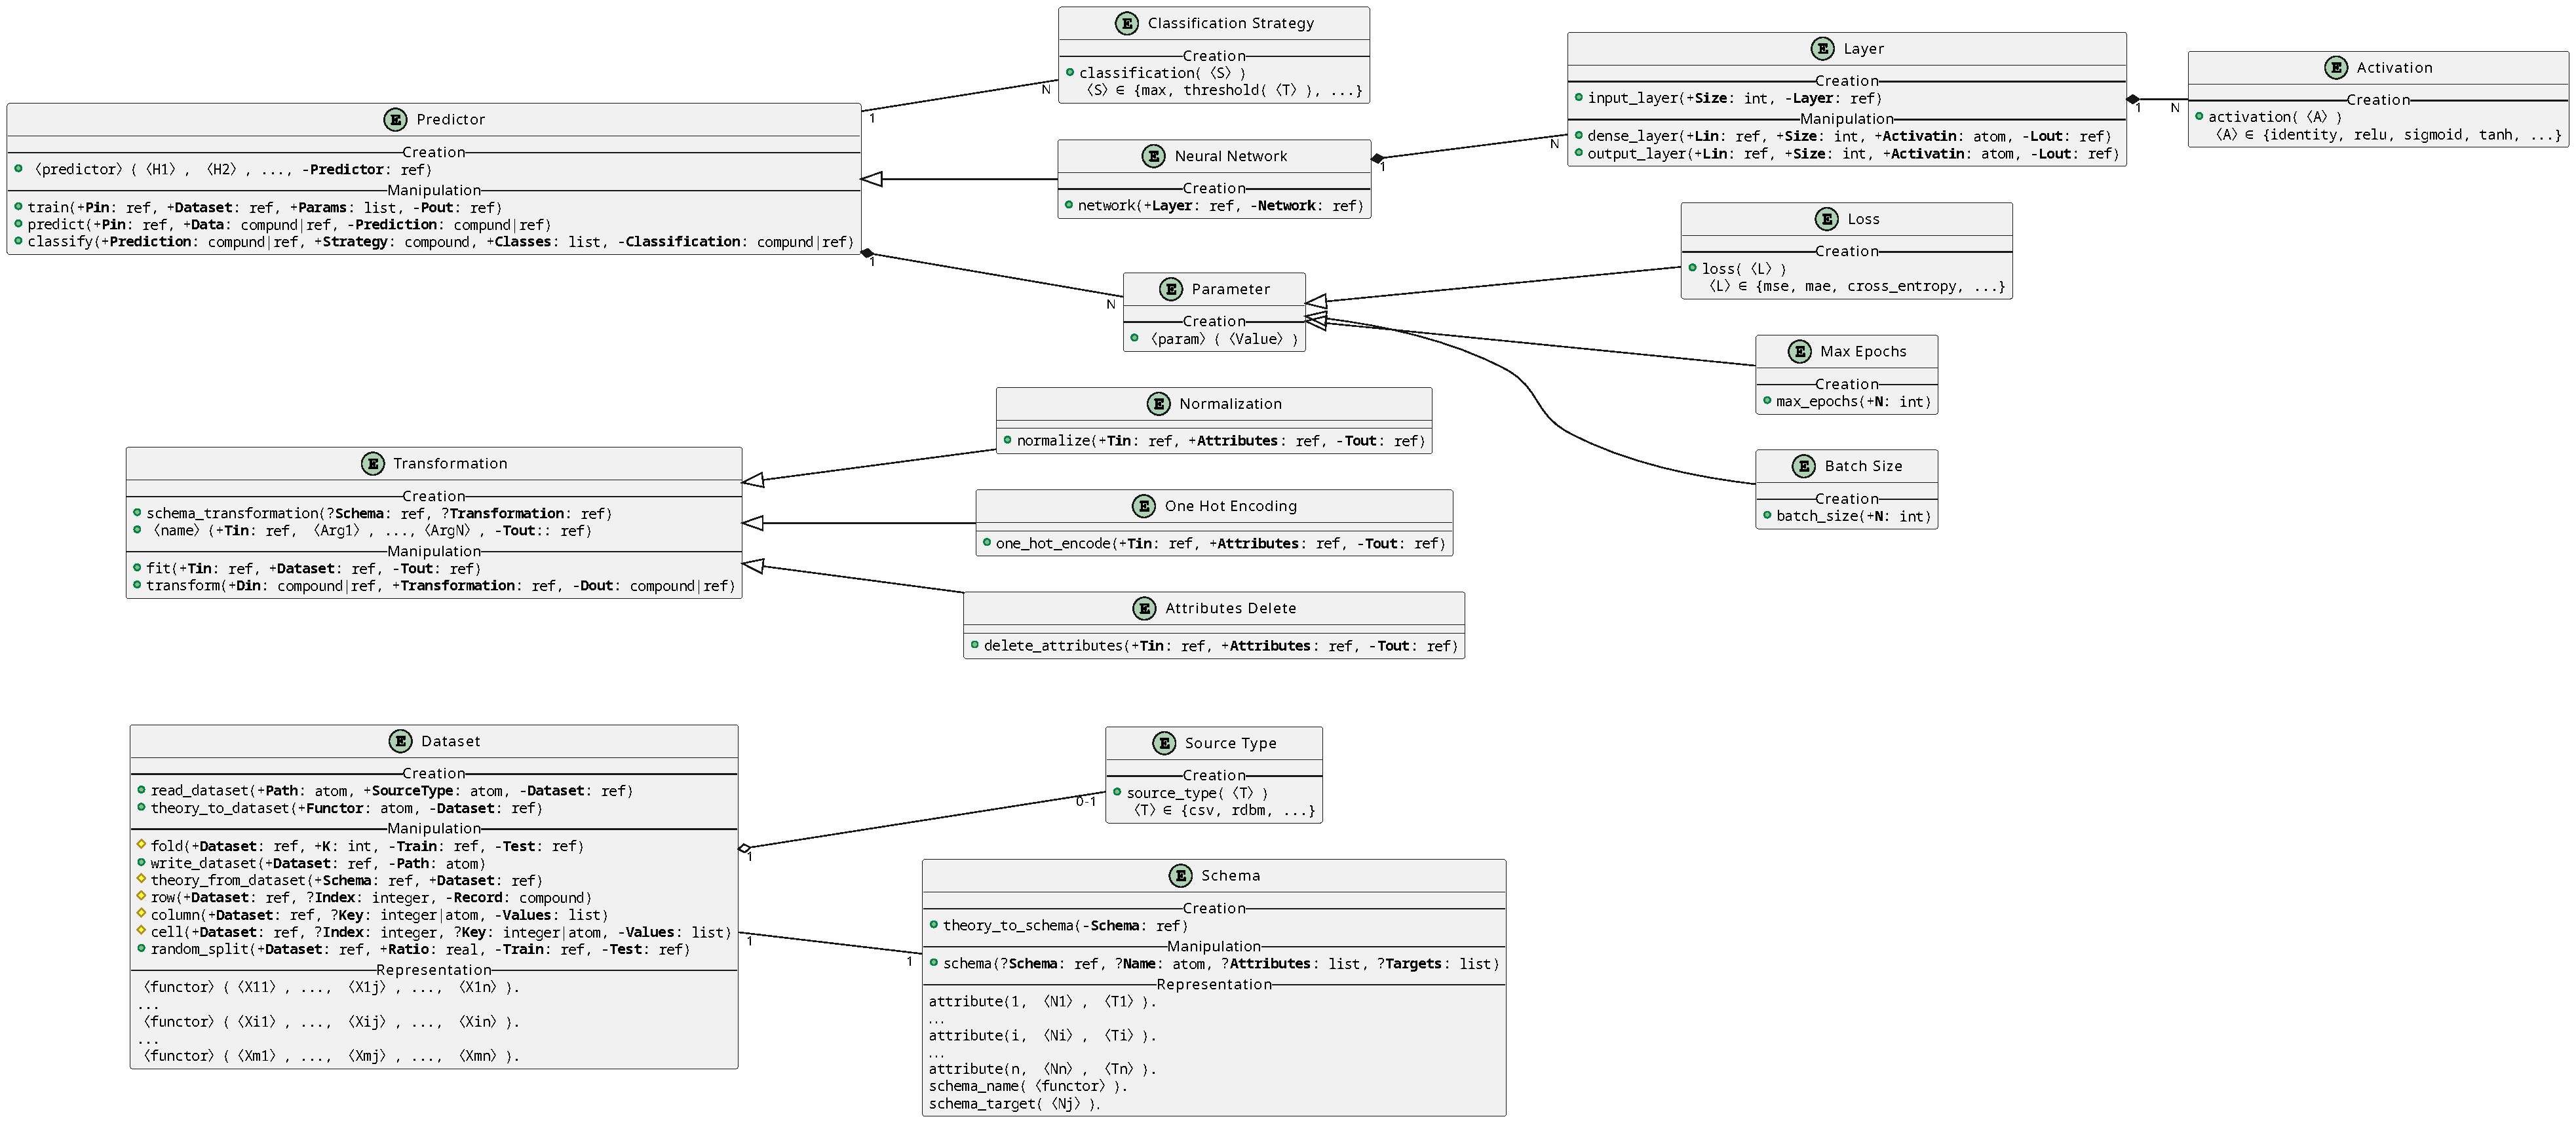
\includegraphics[width=\linewidth]{figures/entities.pdf}
    %
    \begin{itemize}
        \item 4 main kinds of entities: Schema, Dataset, Transformation, Predictor
        %
        \begin{itemize}
            \item plus many ancillary ones (e.g. Parameter, Neural Network, Layer)
        \end{itemize}
        \item many predicates supporting their creation an manipulation in LP
    \end{itemize}

\end{frame}
%\\\\\\\\\\\\\\\\\\\\\

\subsection{Technology Selection}

%\\\\\\\\\\\\\\\\\\\\\
\begin{frame}%[allowframebreaks]
    \frametitle{Technology Selection for the JVM}

    
\begin{table}
    \begin{adjustbox}{width=\textwidth,center}
        \begin{tabular}{c||c|c|c|c}
            \textbf{Project} & \textbf{Developer / Funder} & \textbf{Maturity} & \textbf{Development Status} & \textbf{Documentation}
            \\\hline\hline
            \dlfj{} & Konduit/Eclipse Fundation & Beta & Actively Developed & Excellent
            \\\hline
            Smile & Haifeng Li & Stable & Developed & Excellent
            \\\hline
            Neuroph & Zorac Severac & Stable & Maintained & Acceptable
            \\\hline
            TF4J & Google Brain Team & WIP & Developed & Excellent
            \\\hline
            DJL & Amazon Web Services & Alpha & Actively Developed & Good
            \\\hline
            H20 & H20.ai & Stable & Developed & Good
            \\\hline
            Weka & Waikato University & Stable & Developed & Excellent
        \end{tabular}
    \end{adjustbox}
%    \caption{Recap of the analysed technologies and their features}
%    \label{tab:tech-features}
\end{table}

\begin{table}
    \begin{adjustbox}{width=\textwidth,center}
        \begin{tabular}{ c||c|c|c|c|c }
            \textbf{Project} & \makecell{\textbf{Neural} \\ \textbf{networks}} & \makecell{\textbf{Linear} \\ \textbf{Algebra}} & \makecell{\textbf{Dataset} \\ \textbf{pre-processing}} & \makecell{\textbf{Other sorts} \\ \textbf{of predictors}} & \makecell{\textbf{Differential} \\ \textbf{engine}}
            \\\hline\hline
            \dlfj & Yes & Yes & Yes & No & Yes
            \\\hline
            Smile & No & Yes & Yes & Yes & No
            \\\hline
            Neuroph & Yes & No & No & No & No
            \\\hline
            TF4J & Yes & No & No & No & Yes
            \\\hline
            DJL & Yes & Yes & No & No & Yes
            \\\hline
            H20 & Yes & Yes & Yes & Yes & Unknown
            \\\hline
            Weka & Yes & Yes & Yes & Yes & via \dlfj
        \end{tabular}
    \end{adjustbox}
%    \caption{Recap of the analysed technologies and the functionalities they support}
%    \label{tab:tech-functionalities}
\end{table}


\end{frame}
%\\\\\\\\\\\\\\\\\\\\\

\section{Conclusions \& Future works}

%\\\\\\\\\\\\\\\\\\\\\
\begin{frame}%[allowframebreaks]
\frametitle{Conclusions \& Future works}

\begin{block}{Summing up}
    \begin{itemize}
        \item Design a corpus of predicates supporting ``LP calls ML''
        \item Identify key architectural requirements for its implementation
        \item Select technologies and prototype for the JVM
    \end{itemize}
\end{block}

\begin{exampleblock}{Future Works}
    \begin{itemize}
        \item Port \twopkt{} on Python\footnotemark{}, find some ML tech. \& prototype
        \item Complete support for non-neural predictors
        \item Experiment the creation of actual hybrid systems
    \end{itemize}
\end{exampleblock}

\footnotetext{see \url{https://github.com/tuProlog/2ppy}}

\end{frame}
%\\\\\\\\\\\\\\\\\\\\\

%===============================================================================
\section*{}
%===============================================================================
\frame{\titlepage}

%===============================================================================
\section*{\bibname}
%===============================================================================

\setbeamertemplate{page number in head/foot}{}
%\\\\\\\\\\\\\\\\\\\\\
\begin{frame}[t,allowframebreaks,noframenumbering]\frametitle{\refname}
% \begin{frame}[c]\frametitle{\refname}
	\footnotesize
%	\scriptsize
    \bibliographystyle{apalike-AMS}
    % \bibliographystyle{plain}
	\bibliography{cilc-2022-logic-api-ml-talk}
\end{frame}
%\\\\\\\\\\\\\\\\\\\\\

%%%%%%%%%%%%%%%%%%%%%%%%%%%%%%%%%%%%%%%%%%%%%%%%%%%%%%%%%%%%%%%%%%%%%%%%%%%%%%%%
\end{document}
%%%%%%%%%%%%%%%%%%%%%%%%%%%%%%%%%%%%%%%%%%%%%%%%%%%%%%%%%%%%%%%%%%%%%%%%%%%%%%%%
